\newcommand{\modelreality}{Virtuelt Grupperum}
\newcommand{\topicone}{Aalborg PBL}
\newcommand{\topictwo}{Repr\ae{}sentation}
\newcommand{\topicthree}{Eksempel}
\newcommand{\topicfour}{Design}

\newcommand{\implementaras}{\modelreality}
\newcommand{\topictwoe}{Valg af Plugin Typer}
\newcommand{\topicthreee}{Context}

\section*{\modelreality}

\begin{frame}{\modelreality}
\begin{itemize}
	\item Analyse
	
	\begin{itemize}
		\item \topicone
		\item \topictwo
  \end{itemize}
	
	\item \topicfour
	\begin{itemize}

		\item \topictwoe
		\item \topicthreee
	\end{itemize}
	\item Implementation
  \begin{itemize}
		\item Standard Projekt V�rkt�jer
	\end{itemize}

\end{itemize}
\end{frame}

\begin{frame}{\modelreality}{Analyse} 

\begin{center}
\huge Analyse
\end{center}

\end{frame}

\begin{frame}{\modelreality}{\topicone}
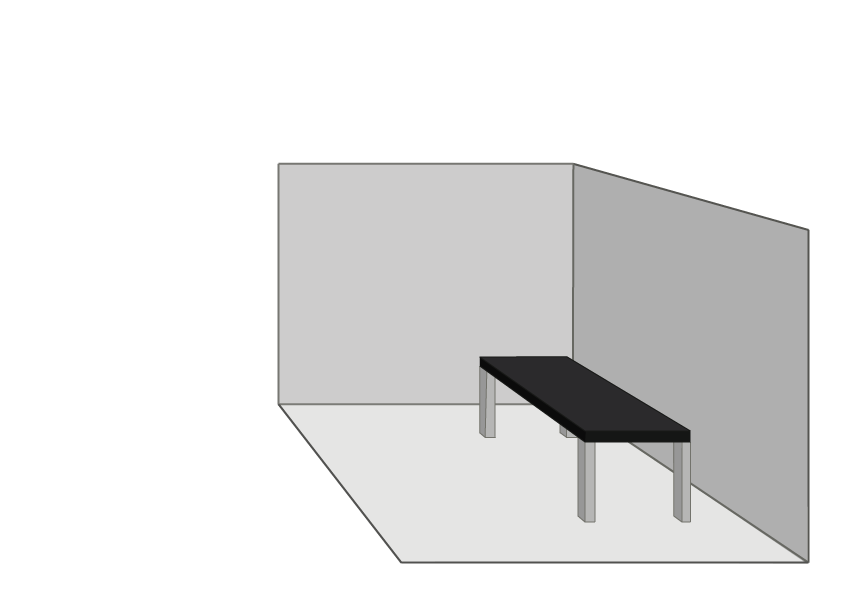
\includegraphics[width=\columnwidth]{input/rasmus/ras5.png}
\end{frame}
\begin{frame}{\modelreality}{\topicone} 
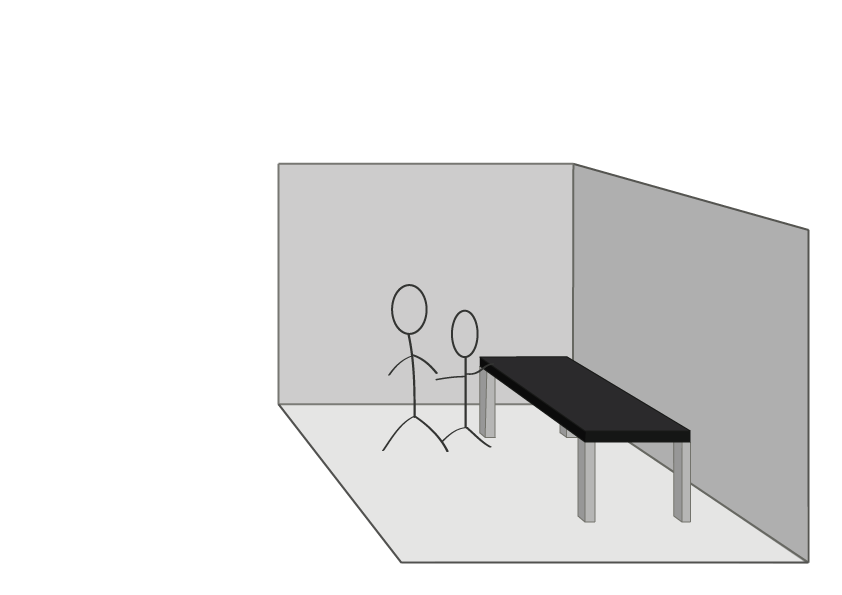
\includegraphics[width=\columnwidth]{input/rasmus/ras4.png}
\end{frame}
\begin{frame}{\modelreality}{\topicone} 
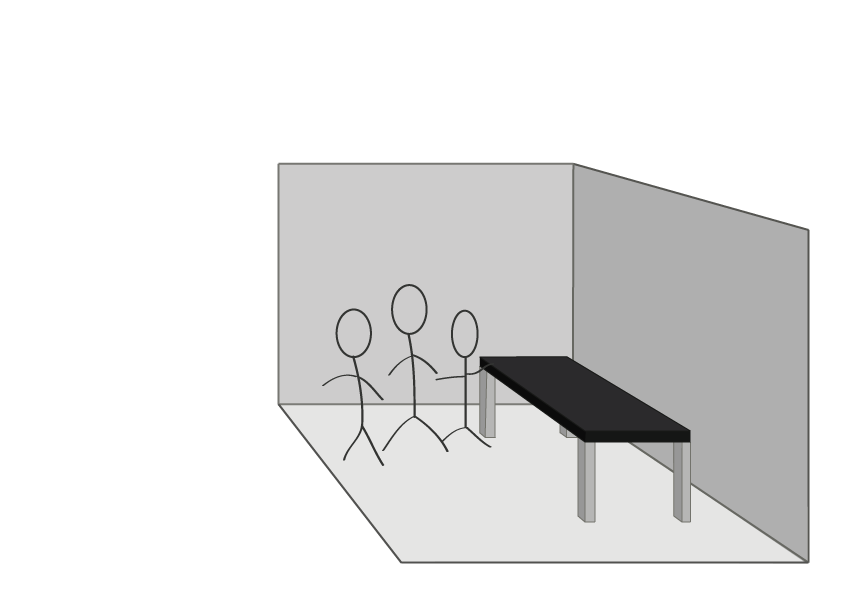
\includegraphics[width=\columnwidth]{input/rasmus/ras3.png}
\end{frame}
\begin{frame}{\modelreality}{\topicone} 
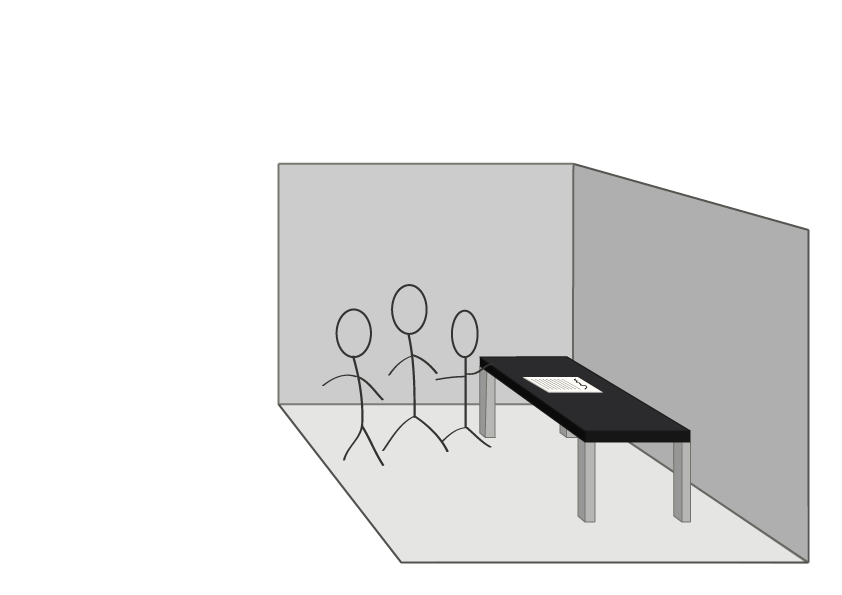
\includegraphics[width=\columnwidth]{input/rasmus/ras2.png}
\end{frame}
\begin{frame}{\modelreality}{\topicone} 
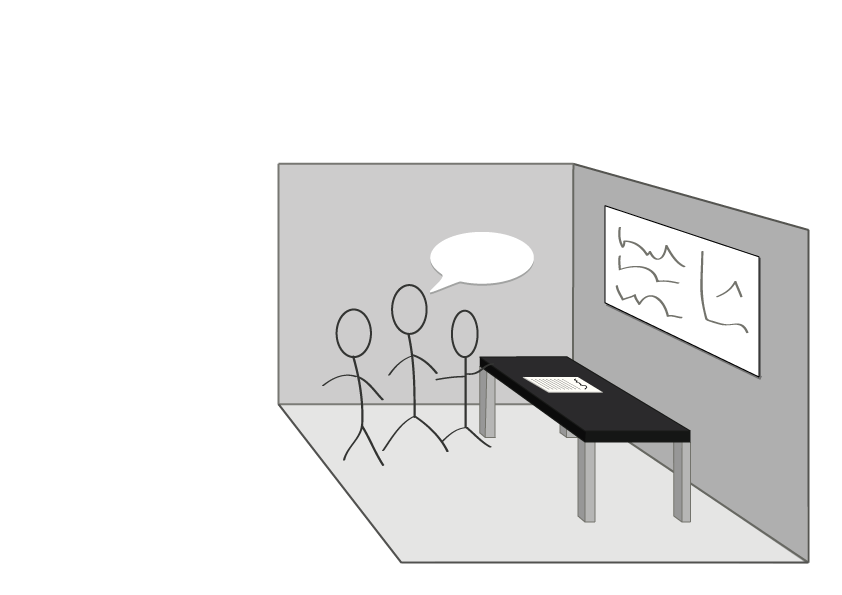
\includegraphics[width=\columnwidth]{input/rasmus/ras1.png}
\end{frame}


\def\freqlist{1,2,3}

\foreach \freq in \freqlist 
{
\begin{frame}{\modelreality}{\topictwo} 
\begin{figure}
\includegraphics[width=\columnwidth]{input/rasmus/two\freq.pdf}
\end{figure}
\end{frame}

} 

\def\freqlist{4,5,6,6a}

\foreach \freq in \freqlist 
{
\begin{frame}{\modelreality}{\topicthree} 
\begin{figure}
\includegraphics[width=\columnwidth]{input/rasmus/two\freq.pdf}
\end{figure}
\end{frame}

} 

\def\freqlist{7,8,9}

\foreach \freq in \freqlist 
{
\begin{frame}{\modelreality}{\topictwo} 
\begin{figure}
\includegraphics[width=\columnwidth]{input/rasmus/two\freq.pdf}
\end{figure}
\end{frame}

} 

\begin{frame}{\modelreality}{\topicfour} 

\begin{center}
\huge Design
\end{center}

\end{frame}


\begin{frame}{\modelreality}{\topicfour} 
\begin{figure}
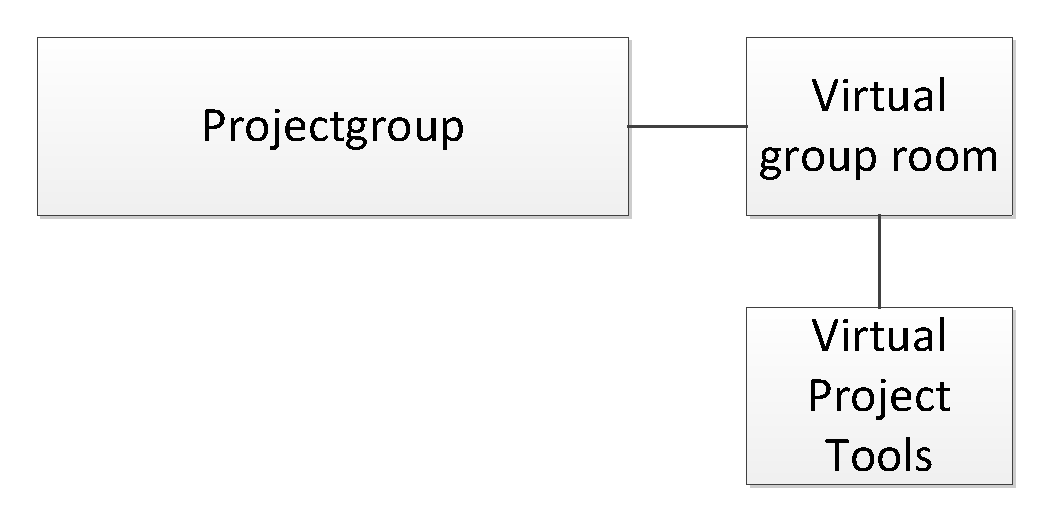
\includegraphics[width=\columnwidth]{input/rasmus/two10.pdf}
\end{figure}
\end{frame}

\begin{frame}{\modelreality}{\topicfour} 
\begin{figure}
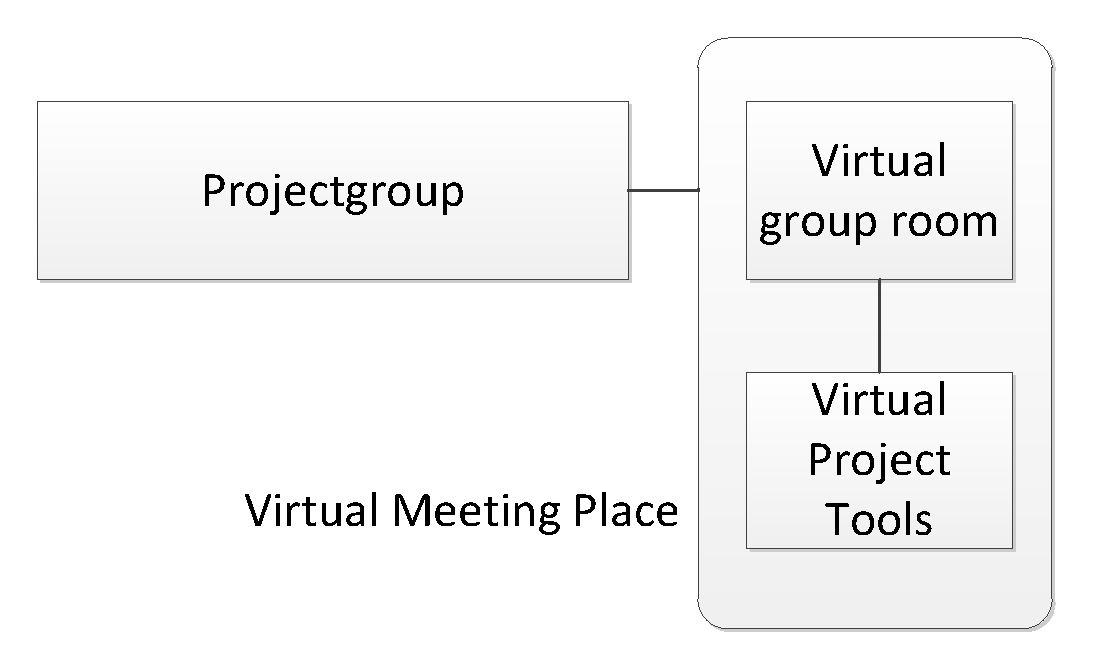
\includegraphics[width=\columnwidth]{input/rasmus/two11.pdf}
\end{figure}
\end{frame}



\def\freqlist{1,1a,2,3,4,5,6,7,7a,8}

\foreach \freq in \freqlist 
{
\begin{frame}{\implementaras} {\topictwoe}
\begin{figure}
\includegraphics[width=\columnwidth]{input/rasmus/three\freq.pdf}
\end{figure}
\end{frame}
}

\def\freqlist{9}

\foreach \freq in \freqlist 
{
\begin{frame}{\implementaras}{\topicthreee} 
\begin{figure}
\includegraphics[width=\columnwidth]{input/rasmus/three\freq.pdf}
\end{figure}
\end{frame}
} 


\begin{frame}{\implementaras}{\topicthreee}
\begin{figure}
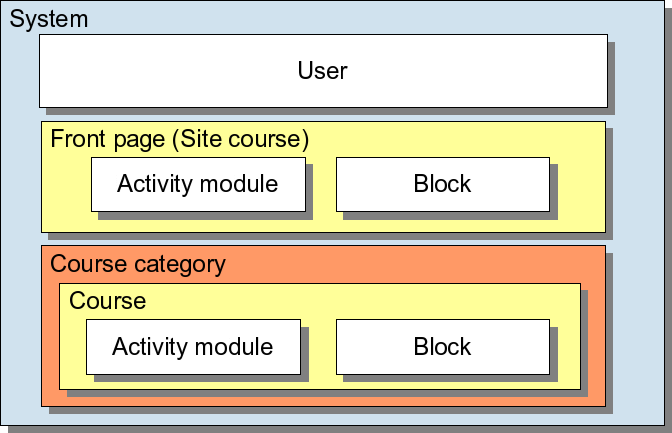
\includegraphics[width=\columnwidth]{input/rasmus/Moodle-contexts.png}
\end{figure}
\end{frame}

\begin{frame}{\implementaras}{\topicthreee}
\begin{figure}
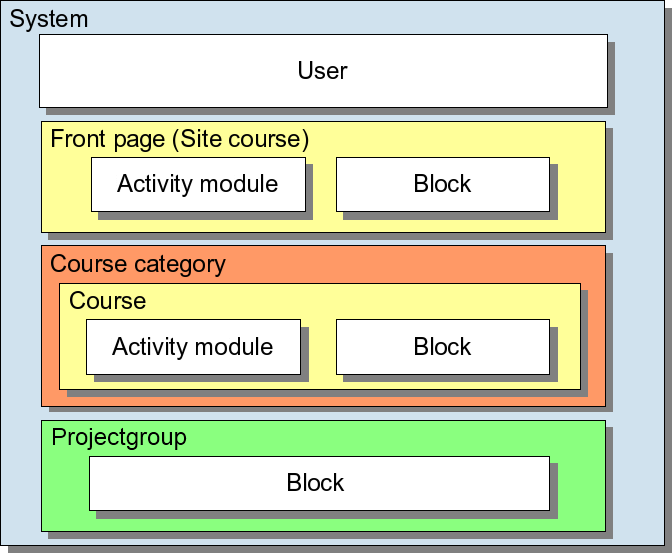
\includegraphics[width=\columnwidth]{input/rasmus/Moodle-contexts-mymoodle.png}
\end{figure}
\end{frame}


\begin{frame}{\modelreality}{Implementation} 

\begin{center}
\huge Implementation
\end{center}

\end{frame}